\subsection{Position changing}
\label{sec:position_change}

To simulate the presence of multiple devices, we generated a list of coordinates on a straight line, and dinamically assigned the right position to each device. In figure \ref{fig:positions} is shown an example of how positions are dinamically reassigned, using our testbed mobile application to test Fast Broadcast algorithm.

Suppose we have four devices, let's called them A, B, C and D, and suppose also we have eight different positions. At the beginning, we have A, B, C and D assigned rispectively on positions 1, 2, 3 and 4. At a certain moment device A sends an \emph{Alert message} to all the other three devices. As soon as it sends the messages, device A moves to position 5. Other devices compute \textit{Contention Window} and wait for a random time. Let's assume now that device C's timeout occours, so it forwards the message: as required by the algorithm, devices B and D stops themselves from forwarding data too (because they just received the message they were about to forward), and device B also moves from position 2 to position 6, reconsidering the message again after moving. The process continues until last position available is reached.
The first position is assigned as soon as connection setup is completed: the designated \textit{group owner} communicates to each other device the file line from whitch reading it. Supposing $N$ devices are involved in the simulation, when one of them has to move to a new position, it will read it $N$ lines below the current one.
With this iterative mechanism we can distribute a certain number of virtual devices on a straight line of arbitrary lenght. 
We also use distance filters to simultae real devices range: once one of the used devices hears a message he souldn't have to hear due to his supposed wireless range, he simply discards it.

\begin{figure}[htbp]
\centering
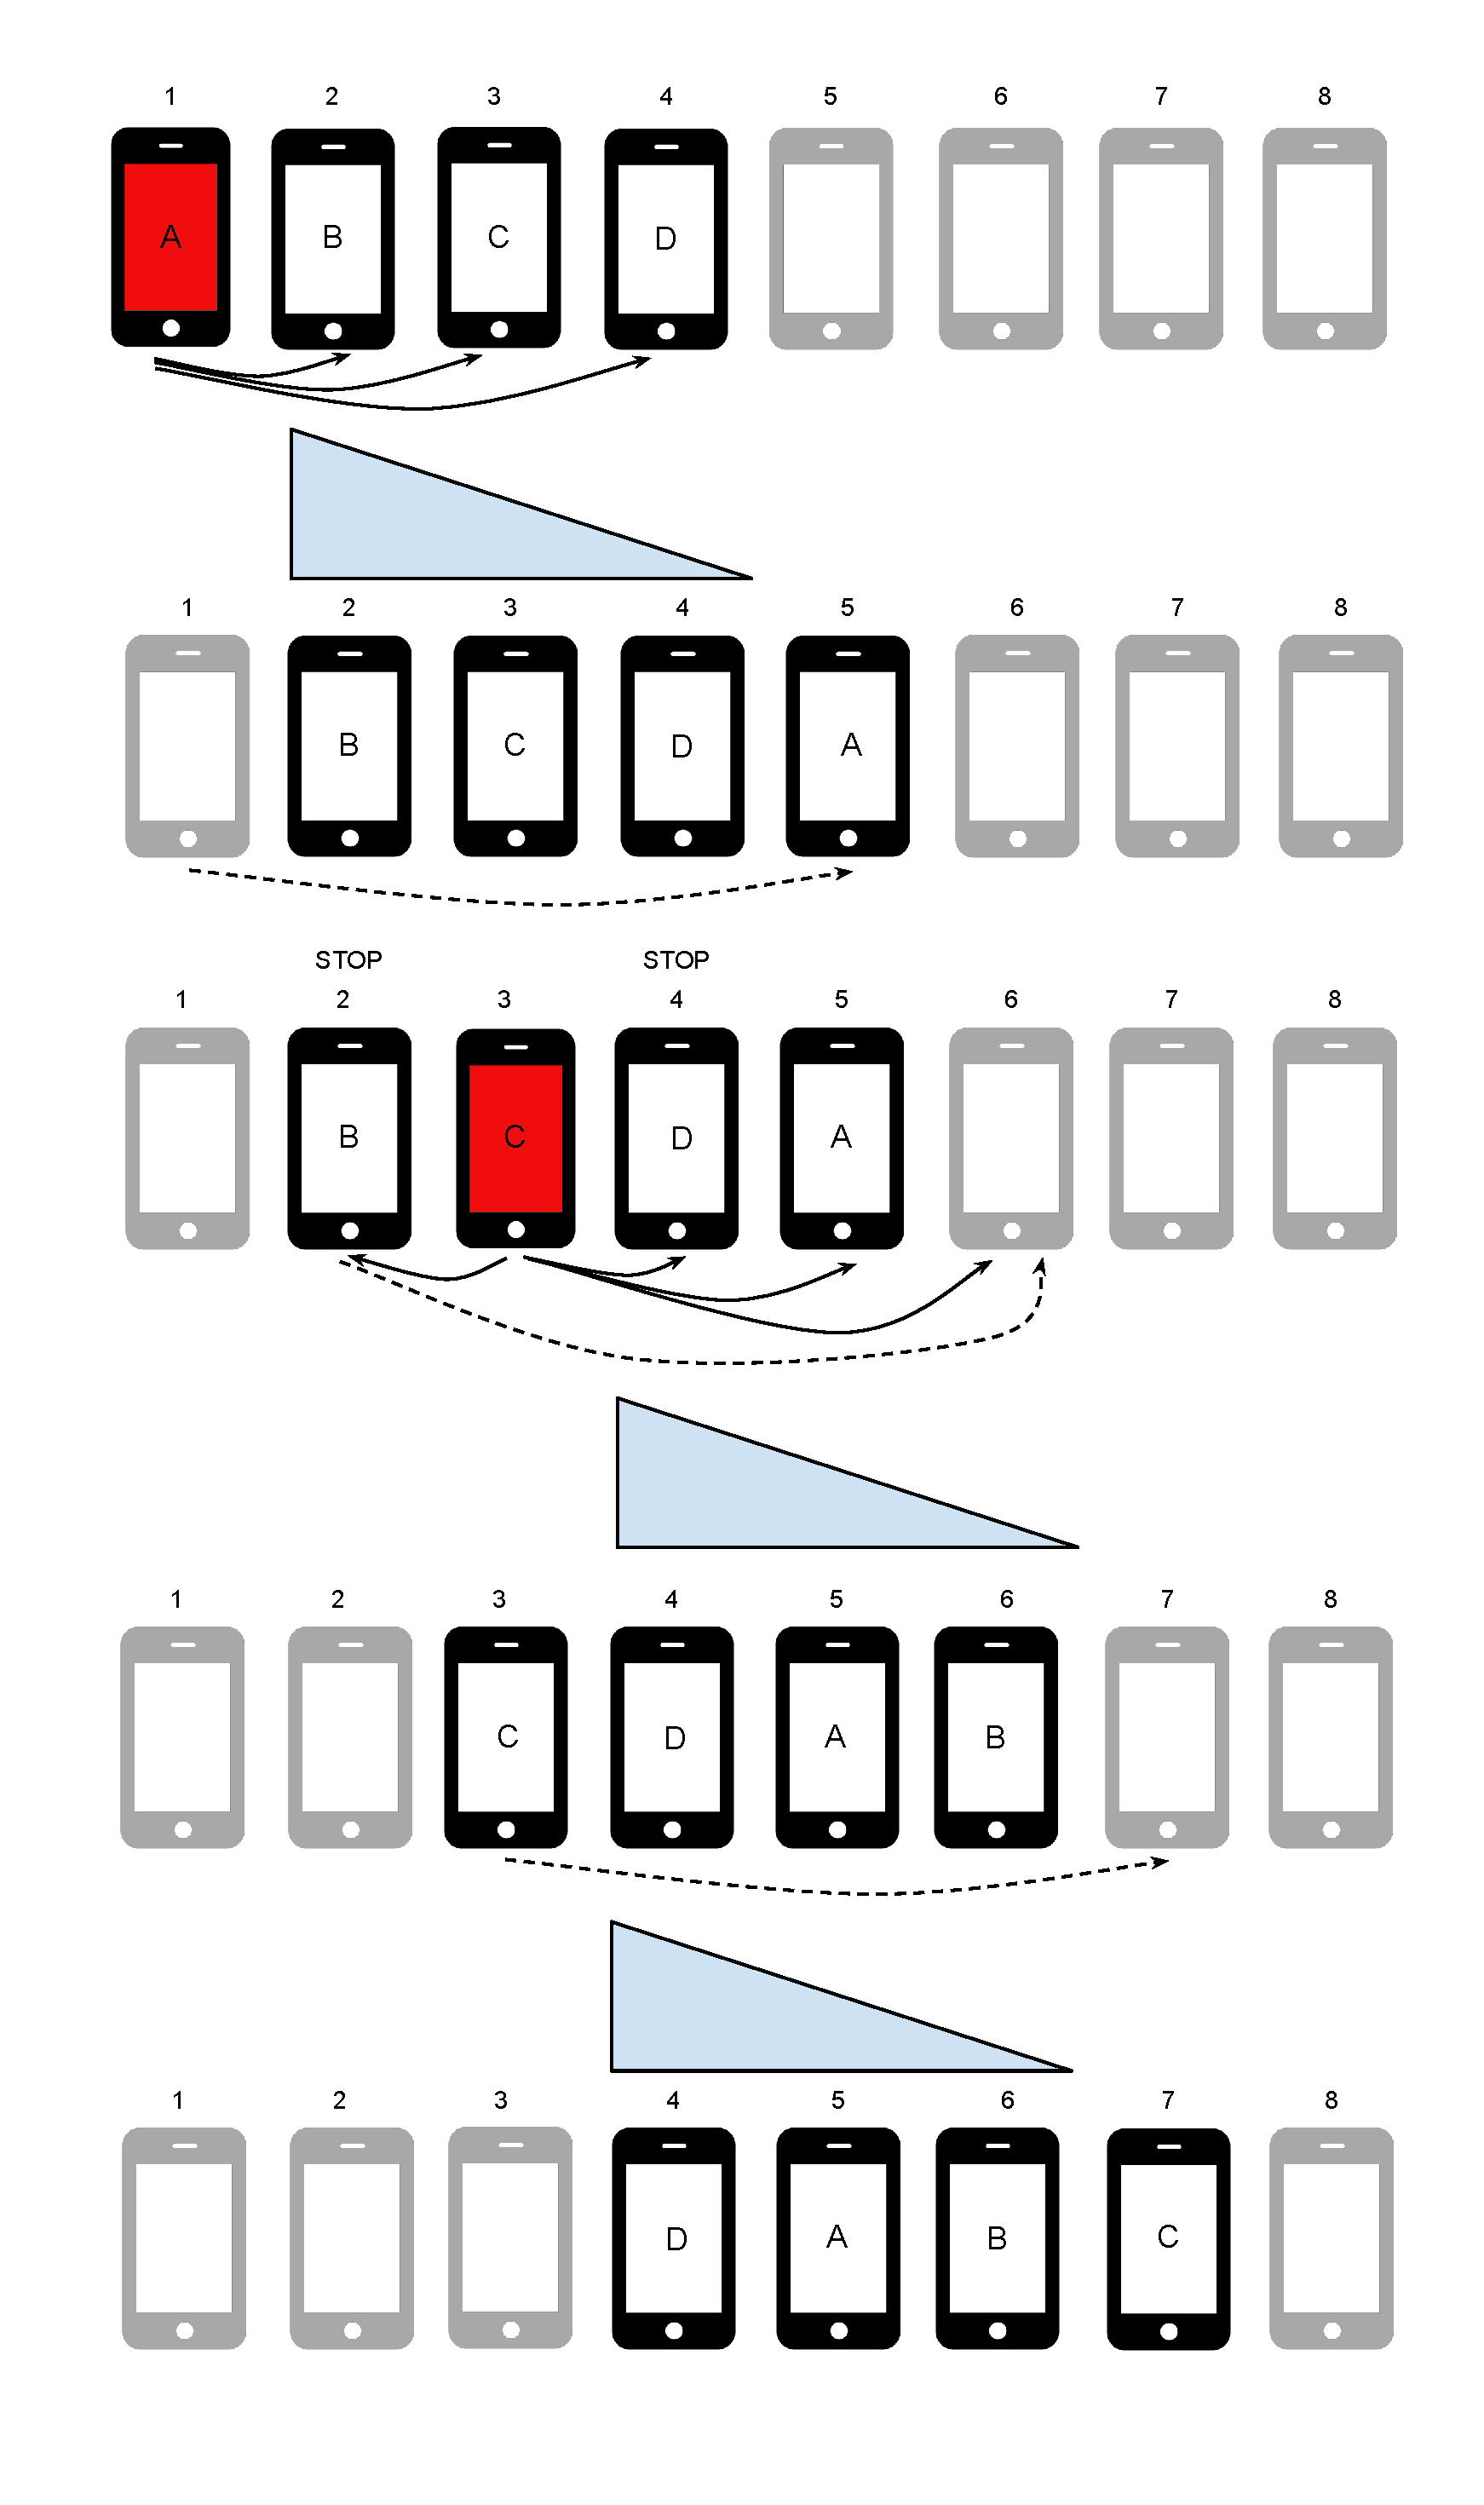
\includegraphics[trim = 15mm 15mm 10mm 10mm ,width=3.6in]{imgs/Positions_1.pdf}
\caption{Devieces position changes}
\label{fig:positions}
\end{figure}
